\chapter{Appendix D}
\labelAppendix{appendix_D}

The server architecture we designed for making our entanglement resource remotely accessible for data acquisition experiments was built around Thorlabs' host-controller communications APT protocol~\cite{thorlabs_apt}. The protocol provides a way to programmatically communicate with almost all Thorlabs motion controllers\footnote{Our experiment uses KDC101 - K-Cube Brushed DC Servo Single-Channel Motor Controllers.}. The communication protocol is based on a message structure that always starts with a fixed length, 6-byte message header which, in some cases, is followed by a variable length data packet, which specifies the sundry byte sequences for sundry operations, all communicated over a USB port. In the name of simplicity, we do not use the protocol in this form but instead use an open-sourced functional implementation in python made by YAQ~\cite{yaq}, which provides modularized functions to invoke sundry operations on motion-controllers such as specifying motors and changing the parameters (speed, acceleration etc) of the motors, hiding the fine-grained implementation details of the APT protocol to the user. 

\bigskip
\noindent
For example, the following code snippet packages the byte sequence to be sent from a source port to a destination source that specifies that an operation that homes a motor to its zero position.

\begin{minted}{python}
def mot_move_home(dest: int, source: int, chan_ident: int) -> bytes:
    return _pack(0x0443, dest, source, param1=chan_ident)
\end{minted}

\noindent
Subsequently, the packaged byte sequence can then be communicated over a USB port to execute on some specified motor, with the following prototypical code snippet:

\begin{minted}{python}
 import thorlabs_apt_protocol as apt
 import serial

 # grab motor connected to USB port 0
 port = serial.Serial("/dev/ttyUSB0", 115200, rtscts=True, timeout=0.1)
 port.rts = True
 port.reset_input_buffer()
 port.reset_output_buffer()
 port.rts = False

 # home motor
 port.write(apt.mot_move_home(source=source, dest=dest, chan_ident=chan_ident))
\end{minted}

\noindent
We used the protocol in a similar manner to the above code snippet, and through an \gls{API}, we exposed the relevant higher-order functionalities required to carry out the various projective measurements in our experiment. Our \acs{API} is served by an HTTP Flask server~\cite{flask} locally hosted on a Raspberry Pi 4. The HTTP server communicates with clients \via HTTP requests (GET, POST, PUT); we use GET requests to serve information about the motors, such as the homing parameters, device status, etc to a client that makes such a request. Similarly, PUT requests are used by clients to update the aforesaid parameters on the motors. And lastly, POST requests are used by clients to start the execution of moves, such as homing, jog etc. The code snippet below shows an \acs{API} endpoint for requests related to the homing move. The GET request here performs the necessary operations to get the homing parameters from a motor specified through the parameters of the request and returns them to the requesting client:


\begin{minted}{python}
@app.route("/home", methods=["GET", "POST", "PUT"])
def home():
    if request.method == "GET":
        device = int(request.args.get("device", 0))
        port = devices[device]

        if port is None:
            return jsonify({"status": "error", "error": "Device unavailable"}), 500

        for i in range(retries):
            port.write(
                apt.mot_req_homeparams(source=source, dest=dest, chan_ident=chan_ident)
            )

            unpacker = apt.Unpacker(port)
            for message in unpacker:
                if hasattr(message, 'msg') and message.msg == "mot_get_homeparams":
                    sem.release()
                    logging.info(message)
                    return jsonify(message), 200

        return (
            jsonify({"status": "error", "error": "Could not get home parameters"}),
            500,
        )
        ...
\end{minted}

\noindent
Similarly, all the necessary operations were exposed as an endpoint of the API. Once this was accomplished, the entirety of the locally hosted \acs{API} was made accessible through a public URL \via ngrok~\cite{ngrok}, giving remote access to the API. Lastly, we designed a mobile graphical user interface (GUI) with Expo~\cite{expo}, which provides a simple and intuitive way to use the \acs{API} for carrying out user-defined experiments and parameter updating operations. We conclude this appendix by showing a demo of the various screens of mobile GUI in~\refFigureOnly{gui1},~\refFigureOnly{gui2} and~\refFigureOnly{gui3}.

\begin{figure}
	\subfloat[\labelFigure{dashboard1}]
	{
		\fbox{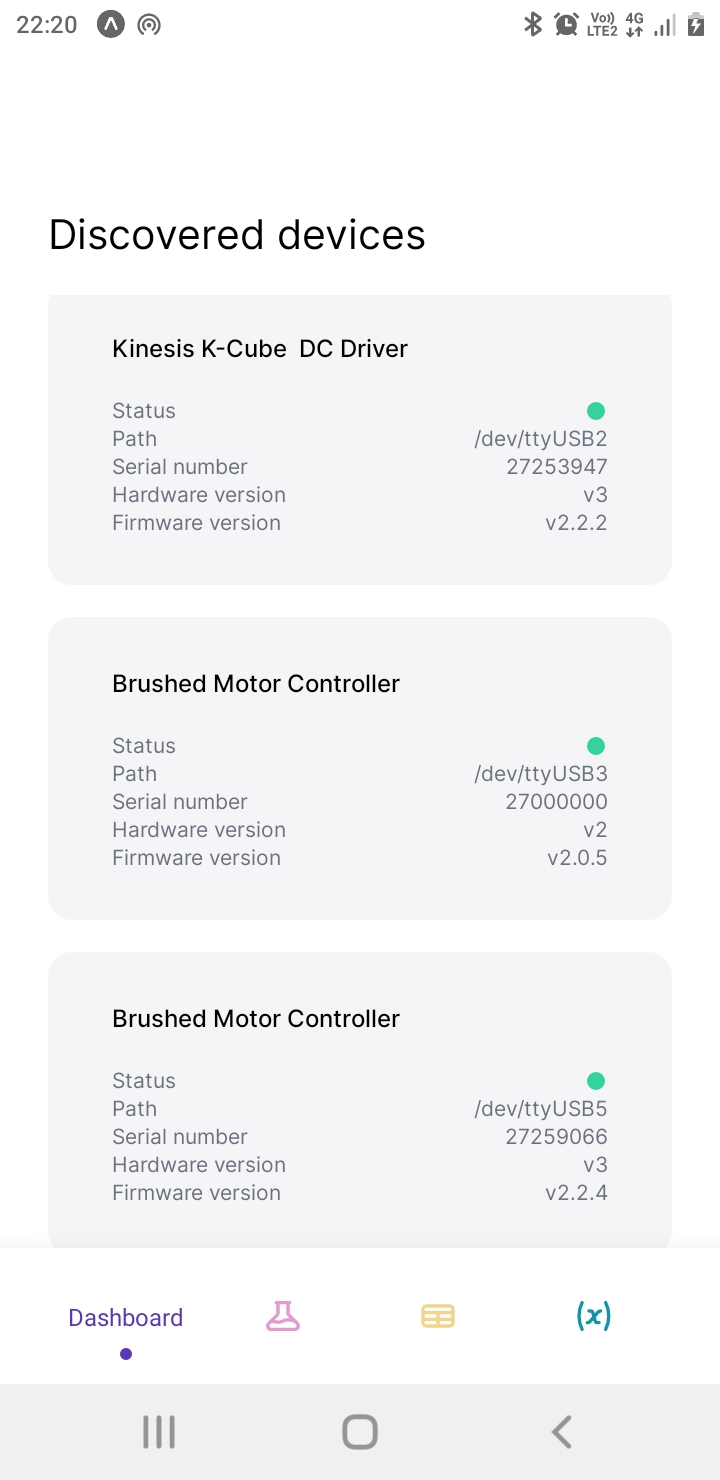
\includegraphics[width=50mm,keepaspectratio]{dashboard1}}
	}
	\subfloat[\labelFigure{dashboard2}]
	{
		\fbox{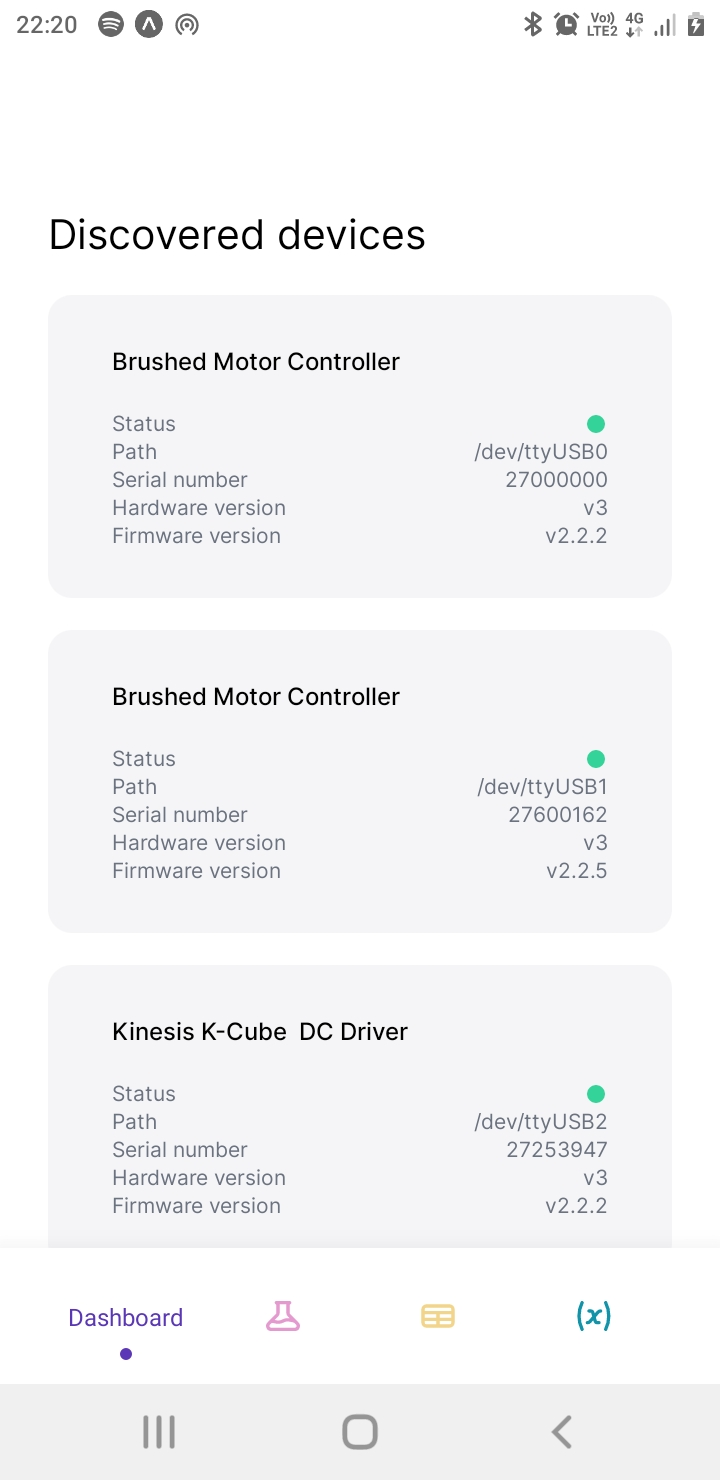
\includegraphics[width=50mm, keepaspectratio]{dashboard2}}
	} \\
	\subfloat[\labelFigure{parameters}]
	{
		\fbox{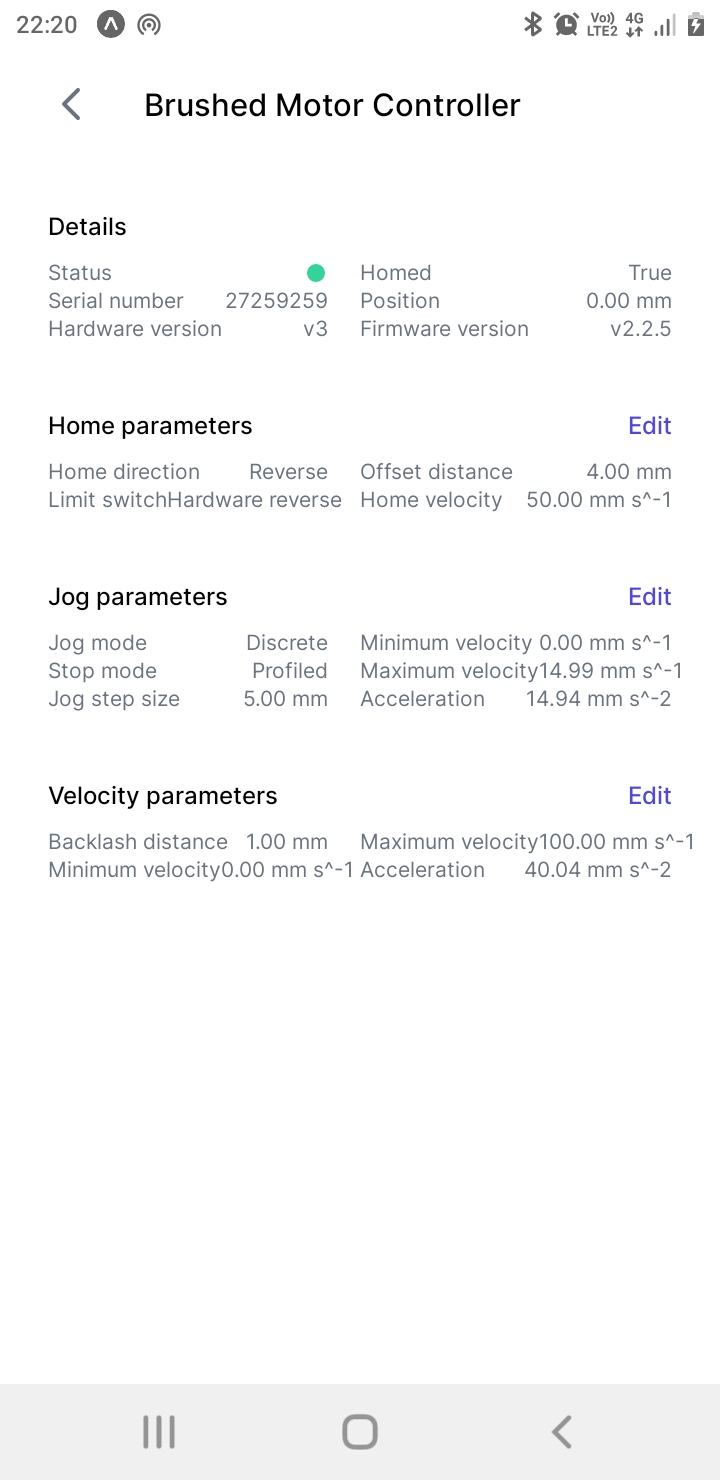
\includegraphics[width=50mm,keepaspectratio]{parameters}}
	} 
	\subfloat[\labelFigure{edit_velocity}]
	{
		\fbox{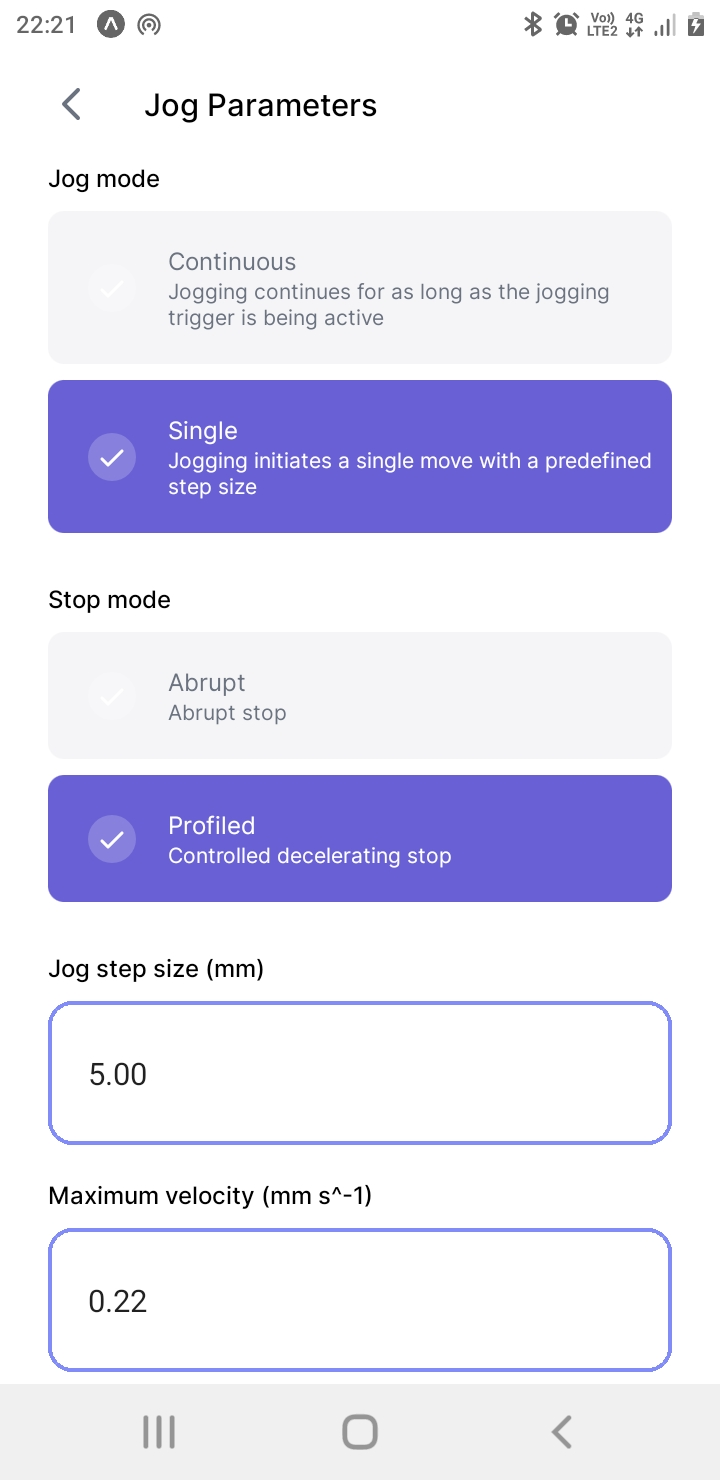
\includegraphics[width=50mm,keepaspectratio]{edit_jog}}
	}
	\caption[Various screens for our mobile graphical user interface for modifying the settings on the motorized devices in our experiments.][6pt]{Various screens for our mobile graphical user interface for controlling our remote source of entanglement: \textbf{(a)},  \textbf{(b)} On the initial load of the GUI, a user gets directed to the dashboard where they can see all the motorized devices and their meta data (online status, hardware etc) accessible by the API. \textbf{(c)} Whenever a user clicks one of the cards, they are directed to a screen with more fine-grained details about that specific device such as jogging parameters, velocity parameters, etc. \textbf{(d)} If a user wishes, it possible to edit the parameters by clicking the edit button next to the type of parameters they wish to change. Where they are taken to a screen with text fields of the editable parameters and the ability to save these changes.} 
	\labelFigure{gui1}
\end{figure}

\begin{figure}
	\subfloat[\labelFigure{composer1}]
	{
		\fbox{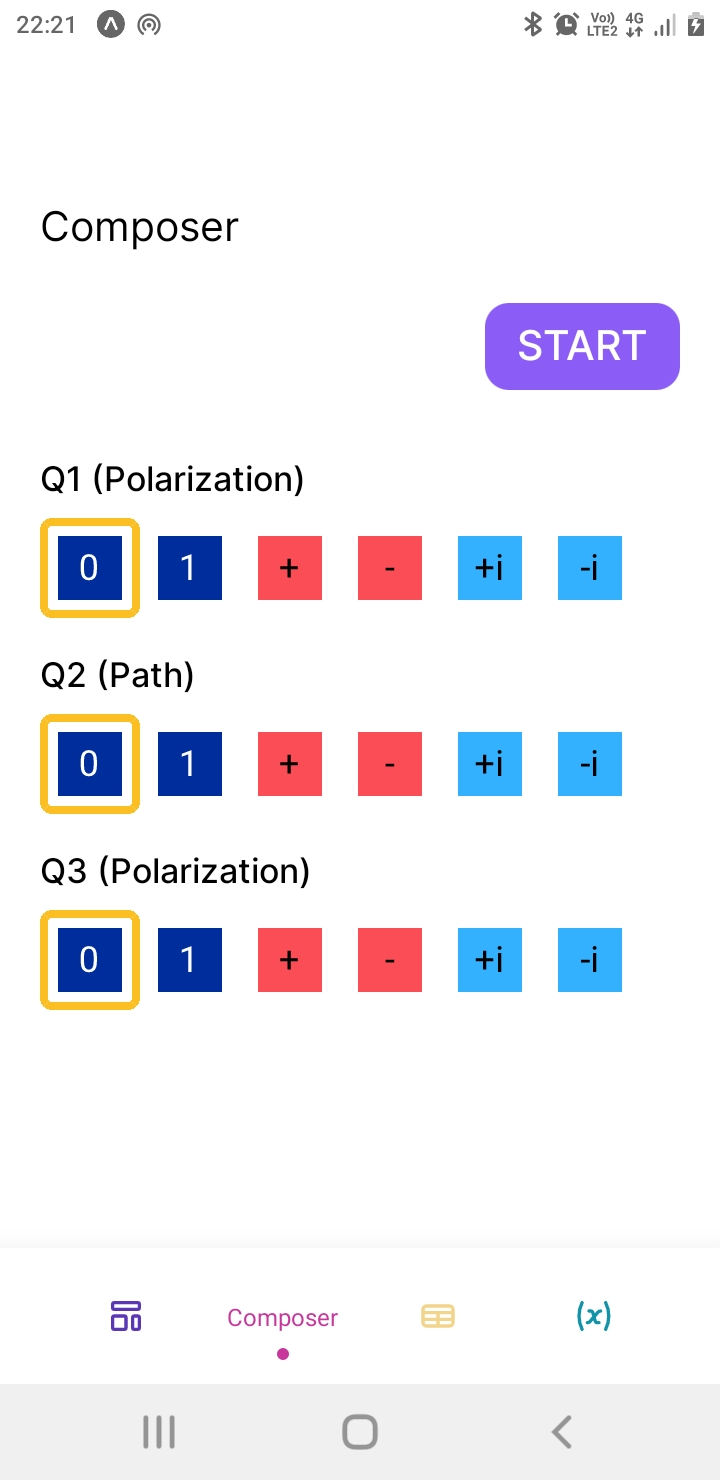
\includegraphics[width=50mm,keepaspectratio]{composer1}
	}}
	\subfloat[\labelFigure{composer2}]
	{
		\fbox{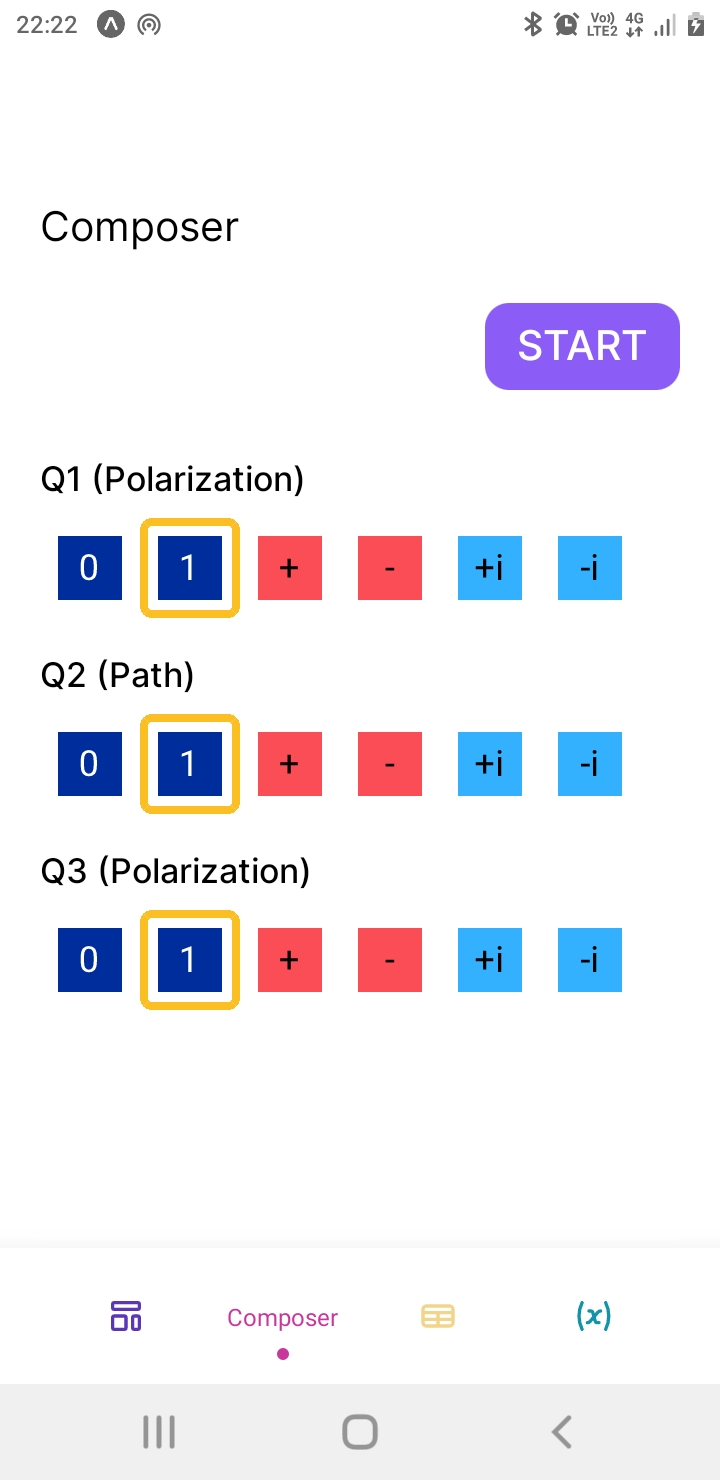
\includegraphics[width=50mm, keepaspectratio]{composer2}}
	} \\
	\subfloat[\labelFigure{move_parameters}]
	{
		\fbox{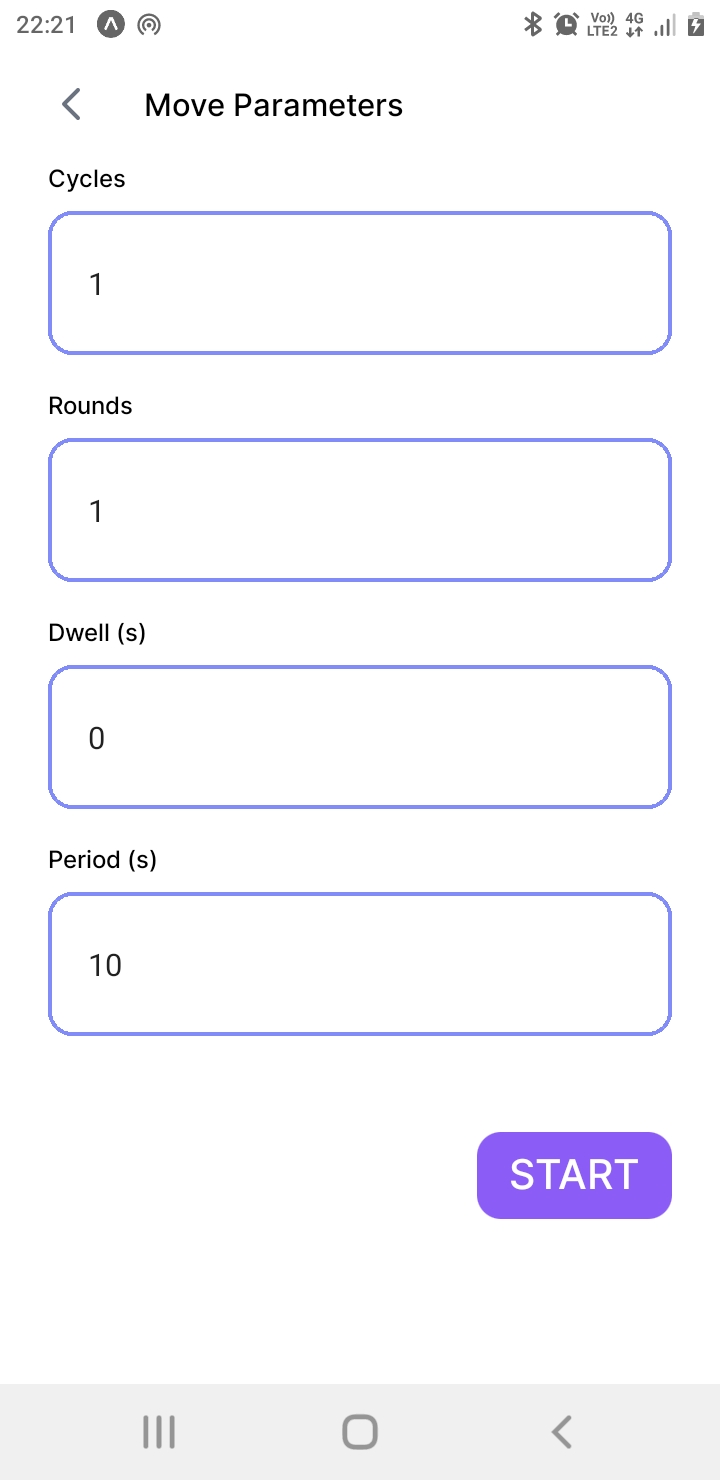
\includegraphics[width=50mm,keepaspectratio]{move_parameters}}
	} 
	\subfloat[\labelFigure{composer_result0}]
	{
		\fbox{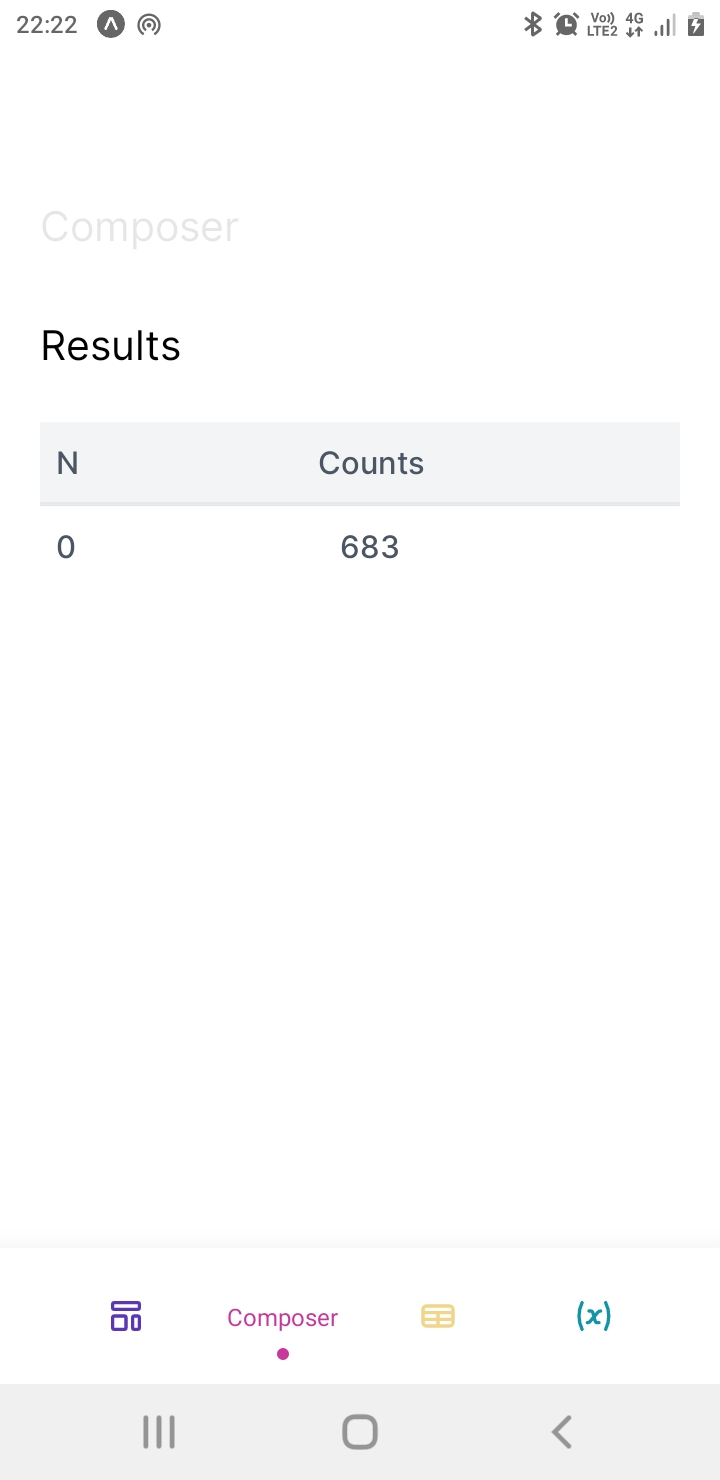
\includegraphics[width=50mm,keepaspectratio]{composer_results}}
	} 
	\caption[Various screens for our mobile graphical user interface for controlling our remote source of entanglement.][6pt]{Various screens for our mobile graphical user interface for controlling our remote source of entanglement. \textbf{(a)}, \textbf{(b)} The composer screen allows a user to set up a simple experiment by specifying the projective measurements on each qubit, with each of the clickable squares representing the measurement basis indicated on the square ${0 = \ket{0}}$, ${1 = \ket{1}}$, ${\pm =(\ket{0} \pm \ket{1})/\sqrt{2}}$ and ${\pm i = (\ket{0}\pm i\ket{1})/\sqrt{2}}$. \textbf{(c)} Once a user is happy with their choice of measurement basis, by clicking start button they can set up data acquisition parameters such as the interval of data collection (period), how many data points are collected (rounds) for the collection interval. Furthermore, they can also specify how many times this experiment is to be repeated (cycles) and the paused between these repeated cycles (dwell). \textbf{(d)} By clicking the start button on the previous screen, the relevant  HTTP requests are made to the API, which are then executed on the motors. Once completed the \acs{API} returns the collected coincidences counts, which are then shown to the user in table format. In this case, the coincidence counts are for the measurement of $\op{1, 1, 1}$} 
	\labelFigure{gui2}
\end{figure}

\begin{figure}
	\subfloat[\labelFigure{sequencer1}]
	{
		\fbox{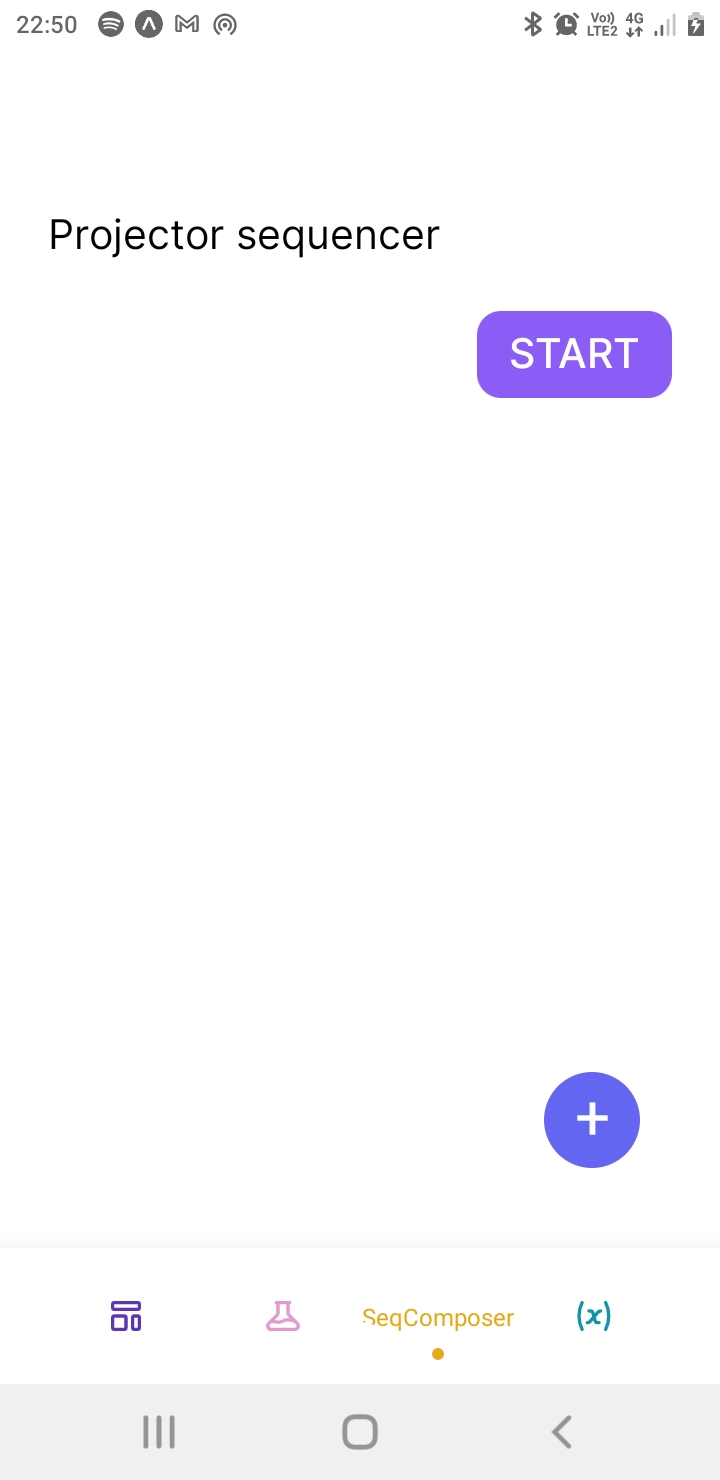
\includegraphics[width=50mm,keepaspectratio]{sequencer1}}
	}
	\subfloat[\labelFigure{move_000}]
	{
		\fbox{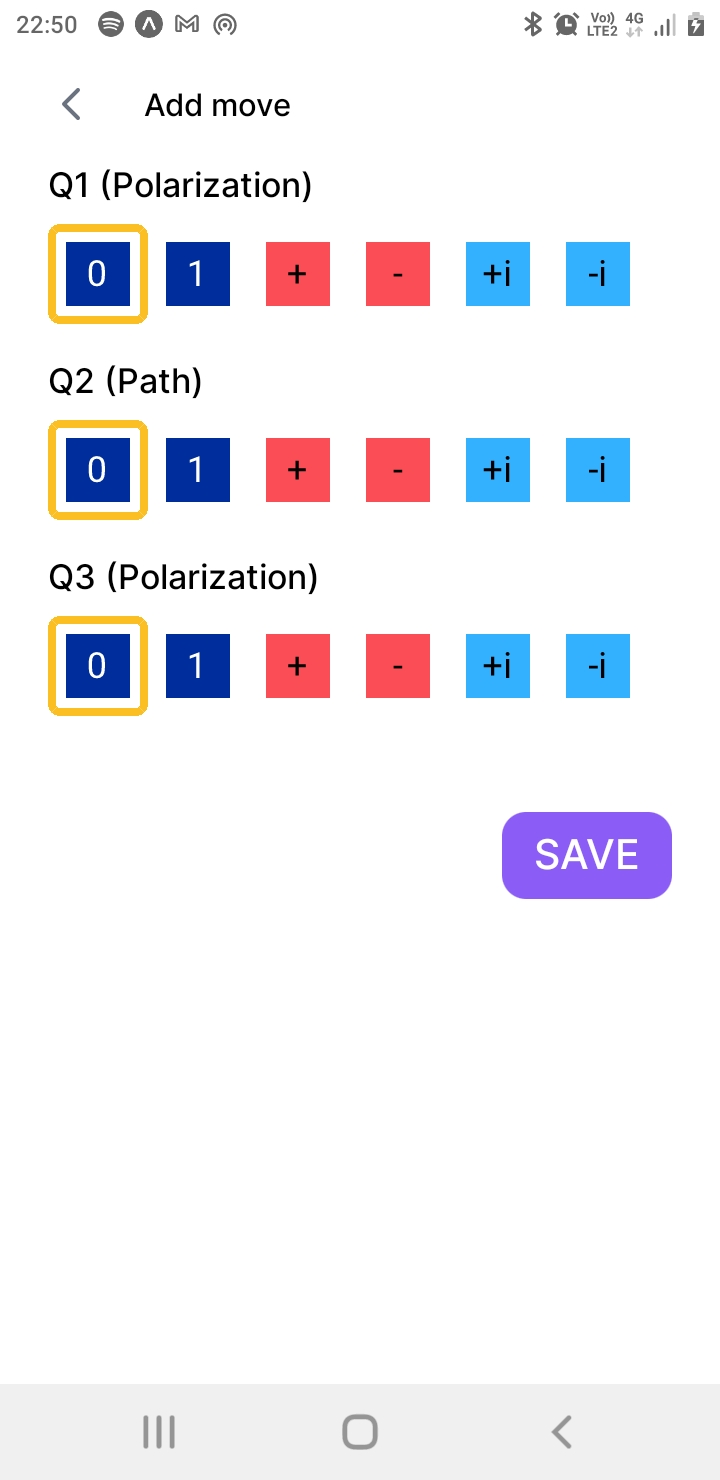
\includegraphics[width=50mm, keepaspectratio]{move_000}
	}} \\
	\subfloat[\labelFigure{move_010}]
	{
		\fbox{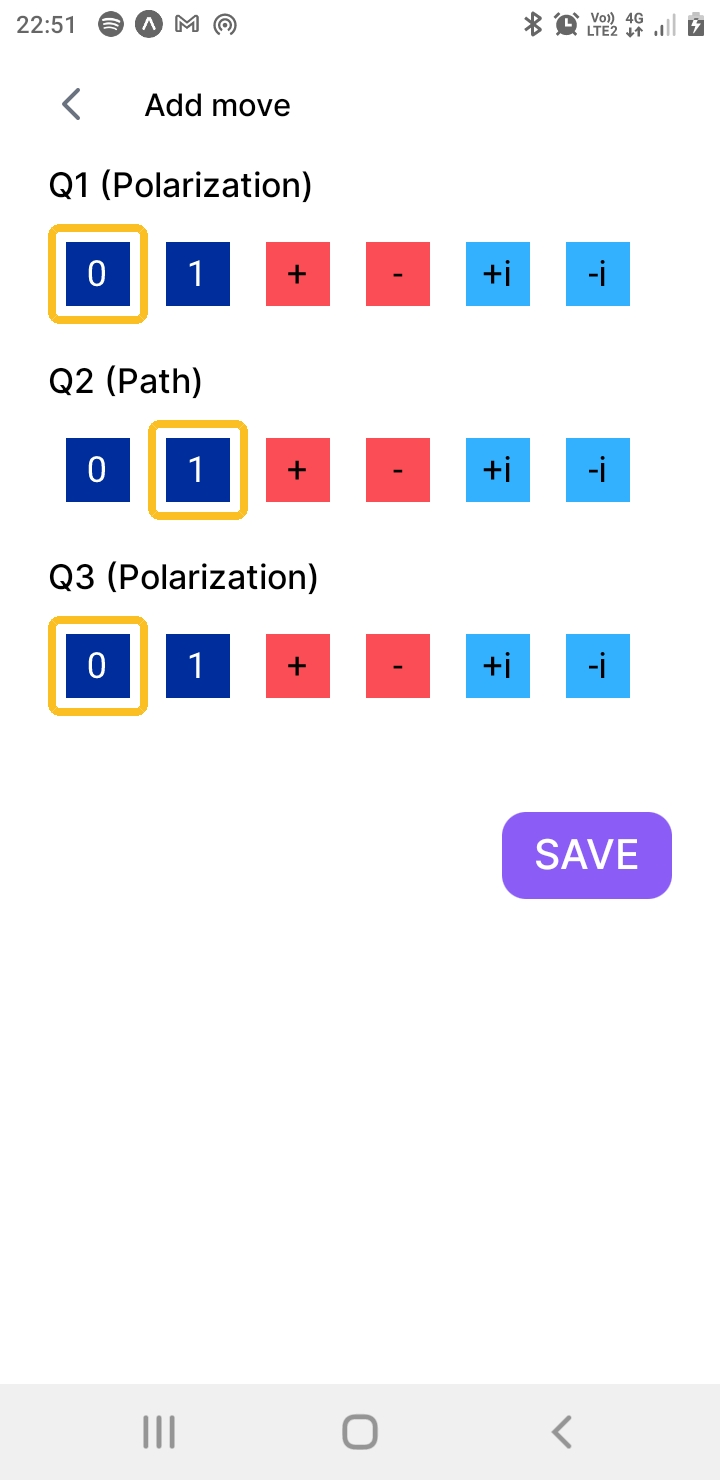
\includegraphics[width=50mm,keepaspectratio]{move_010}
	}}
	\subfloat[\labelFigure{sequencer3}]
	{
		\fbox{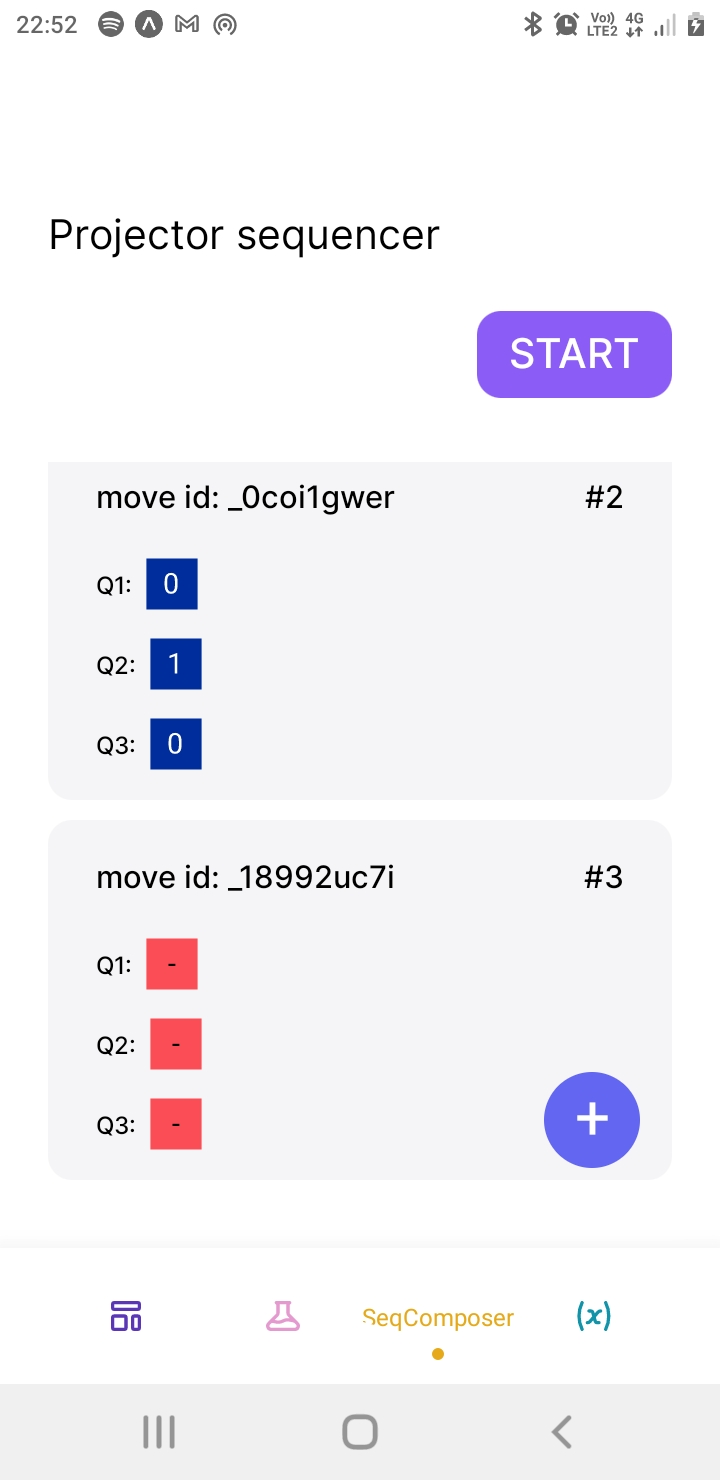
\includegraphics[width=50mm, keepaspectratio]{sequencer3}
	}} 
	\caption[Various screens for our mobile graphical user interface for queueing up a sequence of projective measurements on our remote source of entanglement.][6pt]{Various screens for our mobile graphical user interface for queueing up a sequence of projective measurements on our remote source of entanglement. \textbf{(a)} This screen allows a user to queue up a sequence of projective measurements in a first in first out (FIFO) queue. \textbf{(b)}, \textbf{(c)} By clicking the add button on bottom right, a screen similar to the composer pops up for specifying a projective measurement on each qubit and save it on the queue. \textbf{(d)} The queued projective measurements populate the screen in (a), where queued measurements can be edited and deleted.} 
	\labelFigure{gui3}
\end{figure}


\begin{figure}
	\subfloat[\labelFigure{sequencer4}]
	{
		\fbox{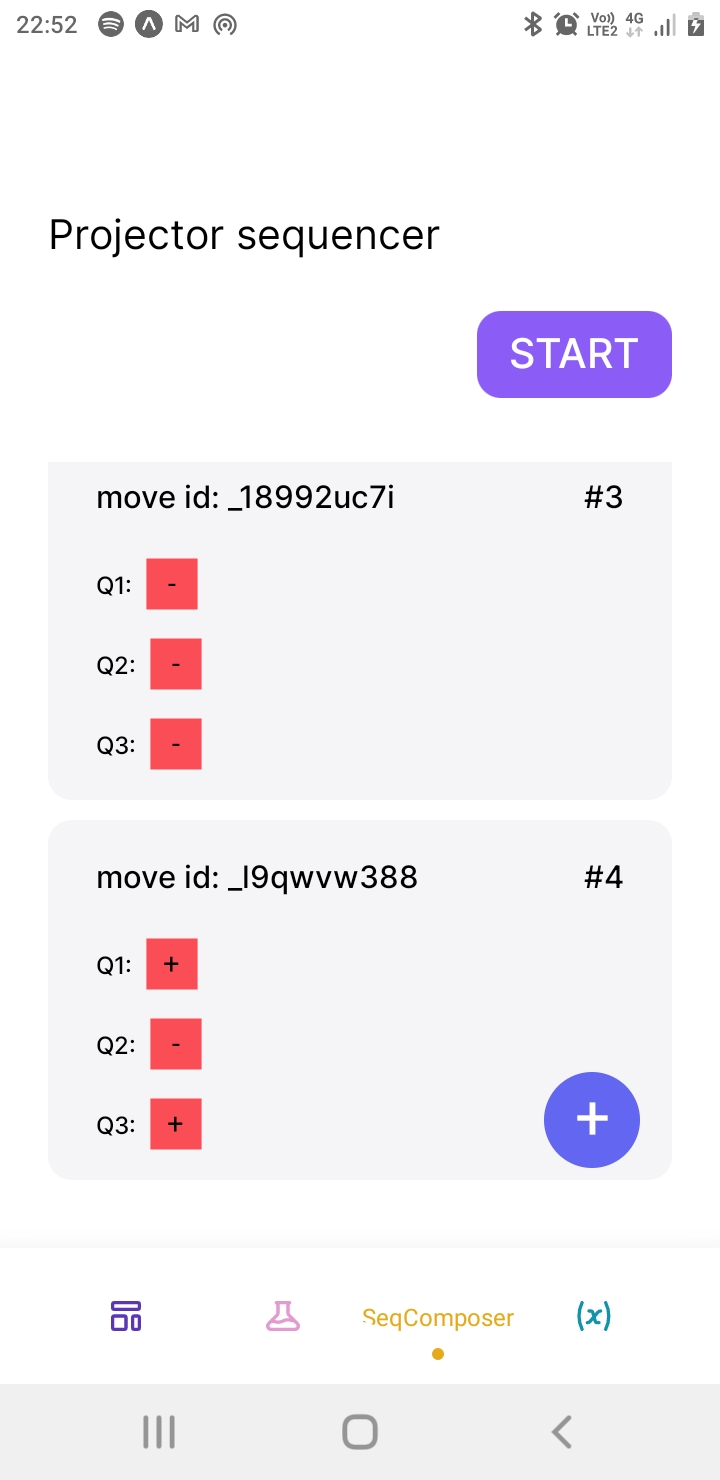
\includegraphics[width=50mm,keepaspectratio]{sequencer4}
	}}
	\subfloat[\labelFigure{edit_measurement}]
	{
		\fbox{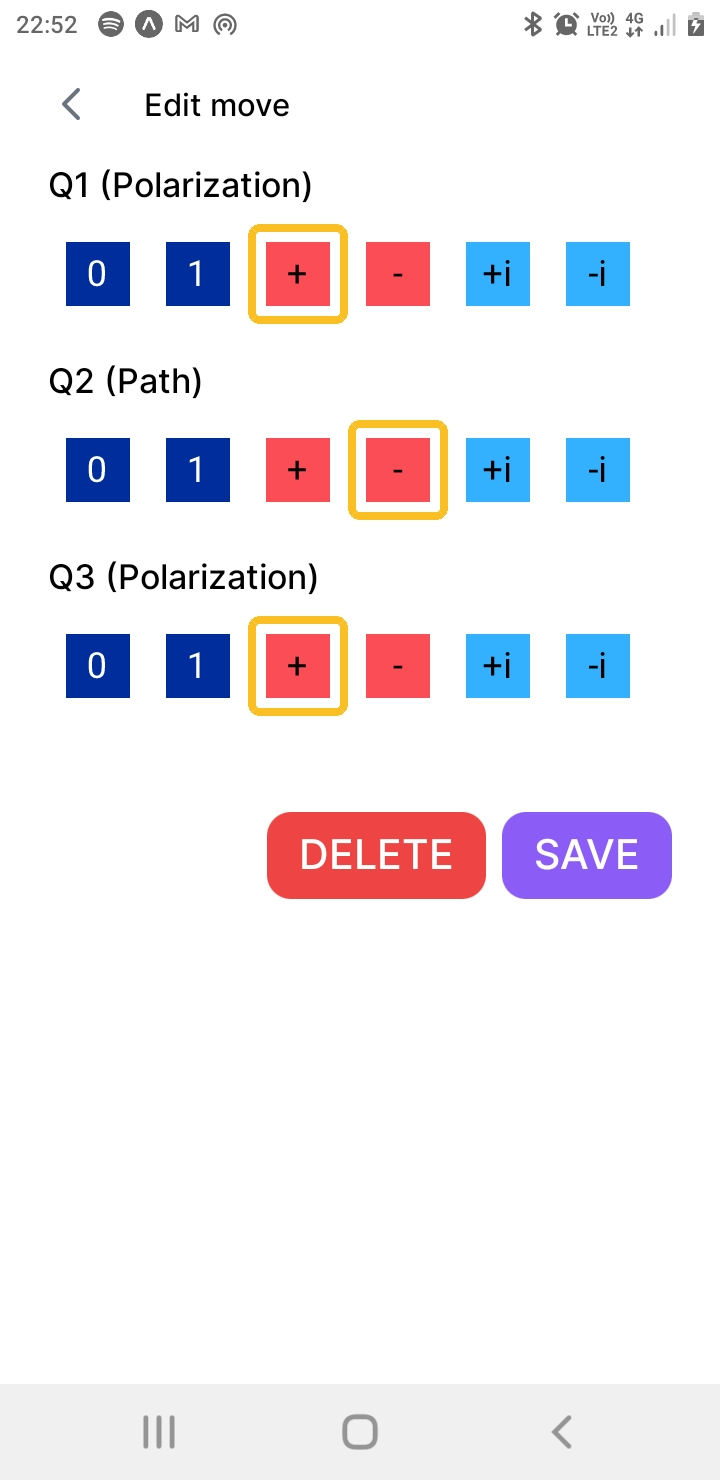
\includegraphics[width=50mm, keepaspectratio]{edit_measurement}
	}} \\
	\subfloat[\labelFigure{loading_state}]
	{
		\fbox{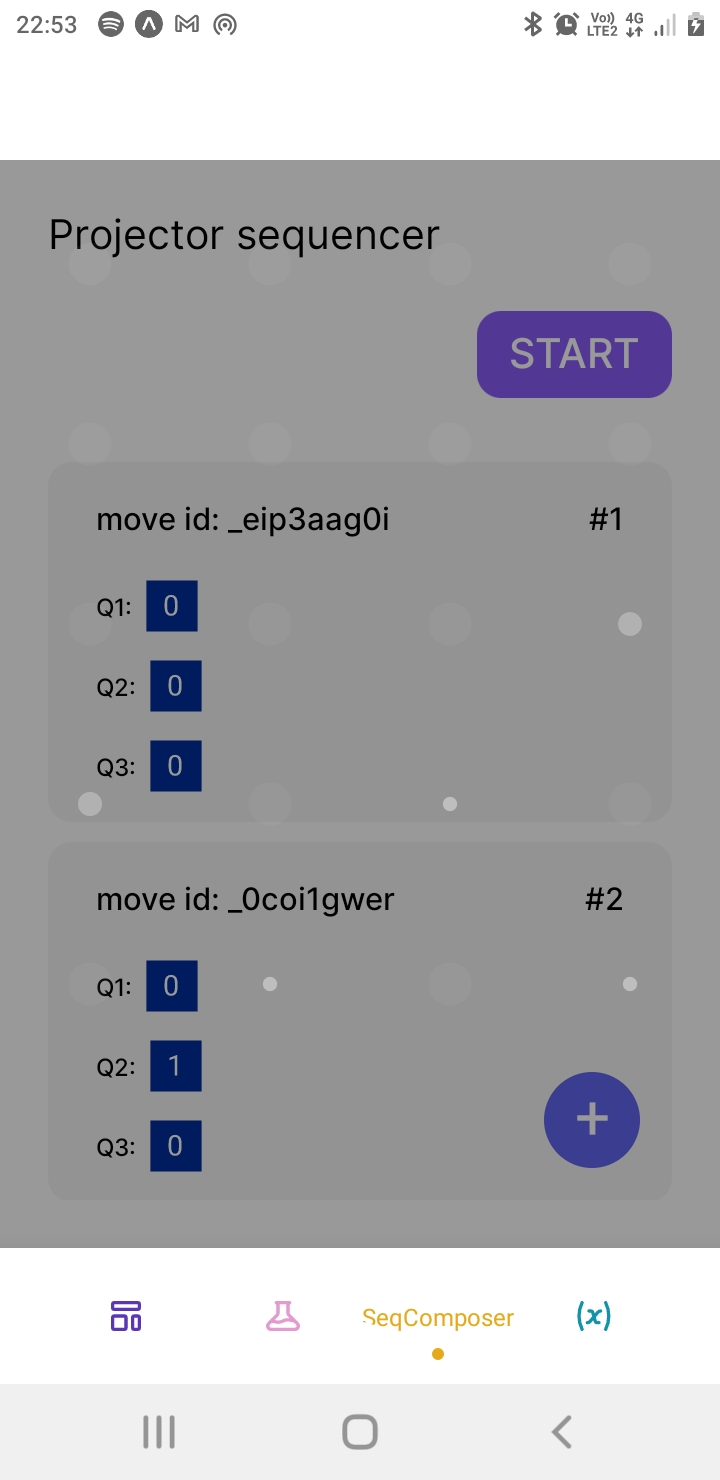
\includegraphics[width=50mm,keepaspectratio]{loading_state}
	}}
	\subfloat[\labelFigure{sequencer_results}]
	{
		\fbox{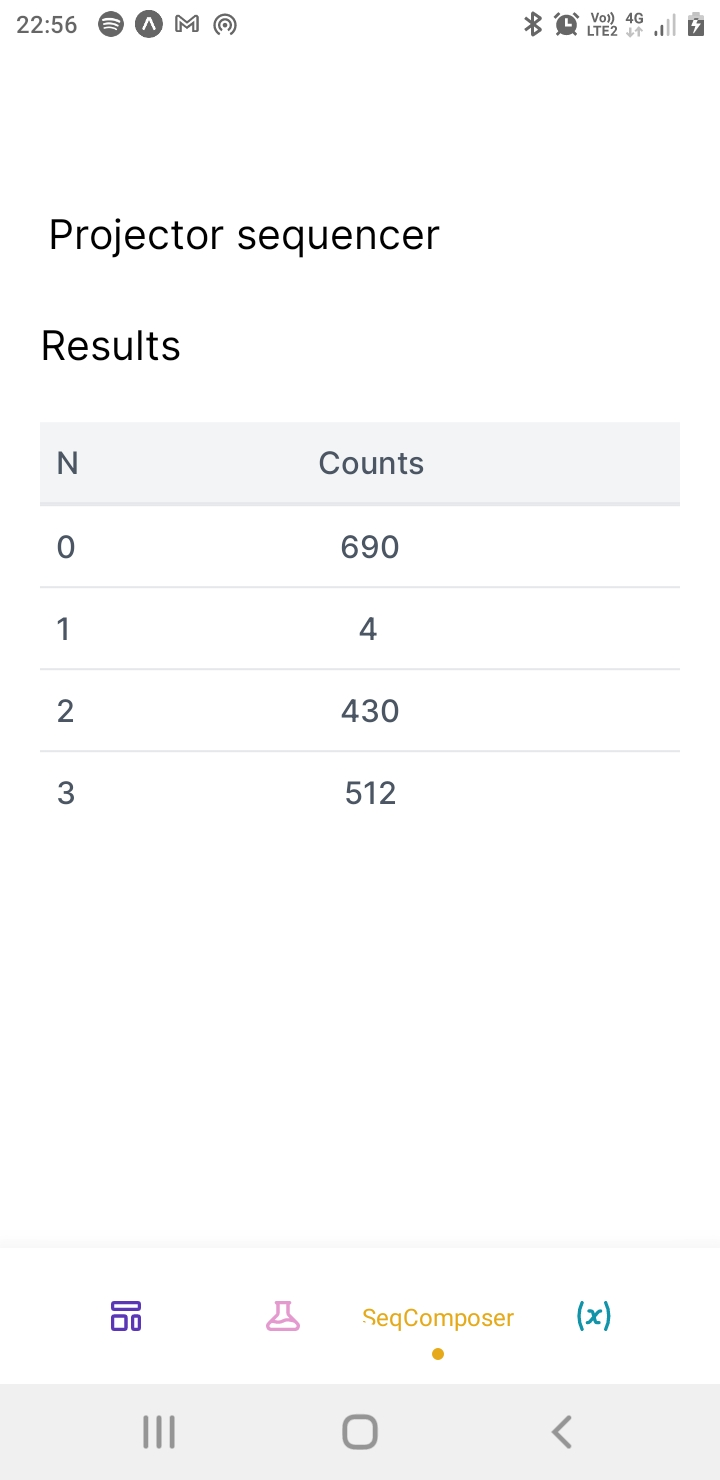
\includegraphics[width=50mm, keepaspectratio]{sequencer_results}
	}} 
	\caption[Various screens for our mobile graphical user interface for editing and executing a sequence of projective measurements on our remote source of entanglement.][6pt]{Various screens for our mobile graphical user interface for editing and executing a sequence of projective measurements on our remote source of entanglement. \textbf{(a)} The queued projective measurements are each assigned a unique ID. \textbf{(b)} By clicking on a specific card, identified by its ID, a screen similar to the composer pops up where the projective measurements can edited or deleted from the queue. \textbf{(d)} Once a user is happy with their queued projective measurements, by clicking the start button screen \textbf{(a)}, they can specify move parameters similar to~\protect\refFigureOnly{gui2} ~\protect\refSubfigureOnly{move_parameters} and start running the queued projective measurements; a loading state is shown. \textbf{(d)} Once finished, the collected double coincidences counts are returned, and are shown to the user in table format, in order of in the order of their execution from the FIFO queue.}
	\labelFigure{gui4}
\end{figure}
